%nag warns a lot about tikzposter.
%\RequirePackage[l2tabu, orthodox]{nag}
\documentclass[blockverticalspace=3cm]{tikzposter}
\input{preamble/packages}
\input{preamble/redac}
\input{preamble/math_basics}
%Decision Theory (MCDA and SC)
\newcommand{\allalts}{\mathscr{A}}
\newcommand{\allcrits}{\mathscr{C}}
\newcommand{\alts}{A}
\newcommand{\dm}{\textcolor{violet}{\ensuremath{i}}}
\newcommand{\model}{\textcolor{cyan}{\eta}}
\newcommand{\allF}{\mathscr{F}}
\newcommand{\allvoters}{\mathscr{N}}
\newcommand{\voters}{N}
\newcommand{\allprofs}{\boldsymbol{\mathcal{R}}}
\newcommand{\prof}{\boldsymbol{R}}
\newcommand{\linors}{\mathscr{L}(\allalts)}
%Thanks to https://tex.stackexchange.com/q/154549
	%\makeatletter
	%\def\@myRgood@#1#2{\mathrel{R^X_{#2}}}
	%\def\myRgood{\@ifnextchar_{\@myRgood@}{\mathrel{R^X}}}
	%\makeatother

%Deliberated Judgment
\newcommand{\props}{\textcolor{red}{T}}
\newcommand{\prop}{\textcolor{red}{t}}
\newcommand{\allargs}{S^*}
\newcommand{\args}{\textcolor{blue}{S}}
\newcommand{\ar}[1][]{%
	\textcolor{blue}{%
		\ifx\\#1\\%
			s
		\else
			s_#1
		\fi%
	}%
}
\newcommand{\ileadsto}{\textcolor{violet}{⇝}}
\newcommand{\ibeatse}{\textcolor{violet}{⊳_\exists}}
\newcommand{\nibeatse}{\textcolor{violet}{⋫_\exists}}
\newcommand{\ibeatsst}{⊳_\forall}
\newcommand{\nibeatsst}{⋫_\forall}
\newcommand{\mleadsto}[1][\eta]{⇝_{#1}}
\newcommand{\mbeats}[1][\eta]{\textcolor{cyan}{⊳_{#1}}}
\newcommand{\ibeatseinv}{⊳_\exists^{-1}}

%Logic
\newcommand{\ltru}{\texttt{T}}
\newcommand{\lfal}{\texttt{F}}


\input{preamble/draw}
\usepackage{tabularx}
\listfiles

%I find these settings useful in draft mode. Should be removed for final versions.
	%Which line breaks are chosen: accept worse lines, therefore reducing risk of overfull lines. Default = 200.
		\tolerance=2000
	%Accept overfull hbox up to...
		\hfuzz=2cm
	%Reduces verbosity about the bad line breaks.
		\hbadness 5000
	%Reduces verbosity about the underful vboxes.
		\vbadness=1300

\title{Studying Deliberated Judgements}
\institute{LAMSADE, Université Paris-Dauphine}
\author{Olivier Cailloux}

\begin{document}
\maketitle[titletotopverticalspace=10cm]

\begin{columns}
	\column{0.4}
		\block{Context and goal of this poster}{
			\begin{tikzpicture}[remember picture,overlay]
				\path (current page.north west) ++(1.5cm, -1cm) node[anchor=north west, inner sep=0] (first) {
					\includegraphics[height=7cm]{LAMSADE95.jpg}
				};
				\path (current page.north) ++(0cm, -1cm) node[anchor=north, inner sep=0] (second) {
					\includegraphics[height=7cm]{Dauphine.jpg}
				};
				\path (current page.north east) ++(-1.5cm, -1cm) node[anchor=north east, inner sep=0] (third) {
					\includegraphics[height=7cm]{PSL.png}
				};
			\end{tikzpicture}
		%
			\begin{tikzpicture}[remember picture,overlay]
				\path (current page.south west) ++(1.5cm, 1.5cm) node[anchor=south west, text width=26cm] {
					Olivier Cailloux and Yves Meinard. \emph{A formal framework for deliberated judgment}. Submitted to Theory and Decision. 
				};
			\end{tikzpicture}
		%
			\begin{itemize}
				\item Internal deliberation facing a decision problem
				\item Considering an individual $i$
				\item Introduce the notion of Deliberated Judgement
				\item Motivate studying it
				\item Sketch how
			\end{itemize}
		}
	\column{0.6}
		\block{Deliberated judgement: a missing conception of “preference”}{
			\begin{itemize}
				\item Descriptive approach
				\begin{itemize}
					\item Observe your epistemic position / choice without interference
				\end{itemize}
				\item Normative approach
				\begin{itemize}
					\item How you ought to reason / choose
					\item Can’t be validated through observation of individuals
				\end{itemize}
				\item \emph{Deliberated} judgement (or preference)
				\begin{itemize}
					\item Your position after having considered all arguments
				\end{itemize}
			\end{itemize}
		}
\end{columns}

\block{Deliberation can change your mind}{
	\newlength{\seplott}
	\setlength{\seplott}{3em}
	\begin{center}
		Choose between L1 and L2, then choose between L3 and L4. Are you sure?
		\framebox{
			\begin{tikzpicture}[grow'=right, sibling distance=3cm, level distance=8cm]
				\path node (l1) {L1} child {
					node {1M €} edge from parent node[above] {100\%}
				};
				\path (l1-1.east) ++ (\seplott, 0) node (ql12) {VS};
				\path (ql12) ++ (\seplott, 0) node[anchor=west] (l2) {L2} child {
					node {0M €} edge from parent node[above] {1\%}
				} child {
					node {1M €} edge from parent node[above right] {89\%}
				} child {
					node {5M €} edge from parent node[below] {10\%}
				};
				\path (l1) ++(40cm, 0) node (l3) {L3} child {
					node {0M €} edge from parent node[above] {89\%}
				} child {
					node {1M €} edge from parent node[below] {11\%}
				};
				\path (l3 -| l3-1.east) ++ (\seplott, 0) node (ql34) {VS};
				\path (ql34) ++ (\seplott, 0) node[anchor=west] (l4) {L4} child {
					node {0M €} edge from parent node[above] {90\%}
				} child {
					node {5M €} edge from parent node[below] {10\%}
				};
			\end{tikzpicture}
		}
	\end{center}
	\mbox{}

	\begin{minipage}{0.6\textwidth}
%		\rule{\textwidth}{1cm}
		\begin{itemize}
			\item First observation (Bernouilli): don’t be content with maximizing (untransformed) expected revenue!
			\item Second observation: $i$ could be intuitively attracted by L1 $\succ$ L2 and L3 $\succ$ L4 (Allais’s problem)
			\item Including Savage
			\item And might change her mind when given a reasoning pro expected utility
			\item “There is, of course, an important sense in which preferences, being entirely subjective, cannot be in error”
			\item … “but in a different, more subtle sense they can be.” (Savage, The Foundations of Statistics)
			\item[⇒]Systematic decision principles might help deliberate
		\end{itemize}
	\end{minipage}%
	\begin{minipage}{0.33\textwidth}%
		\footnotesize
%		\rule{\textwidth}{1cm}
		\centering
		\setlength{\seplott}{3em}
		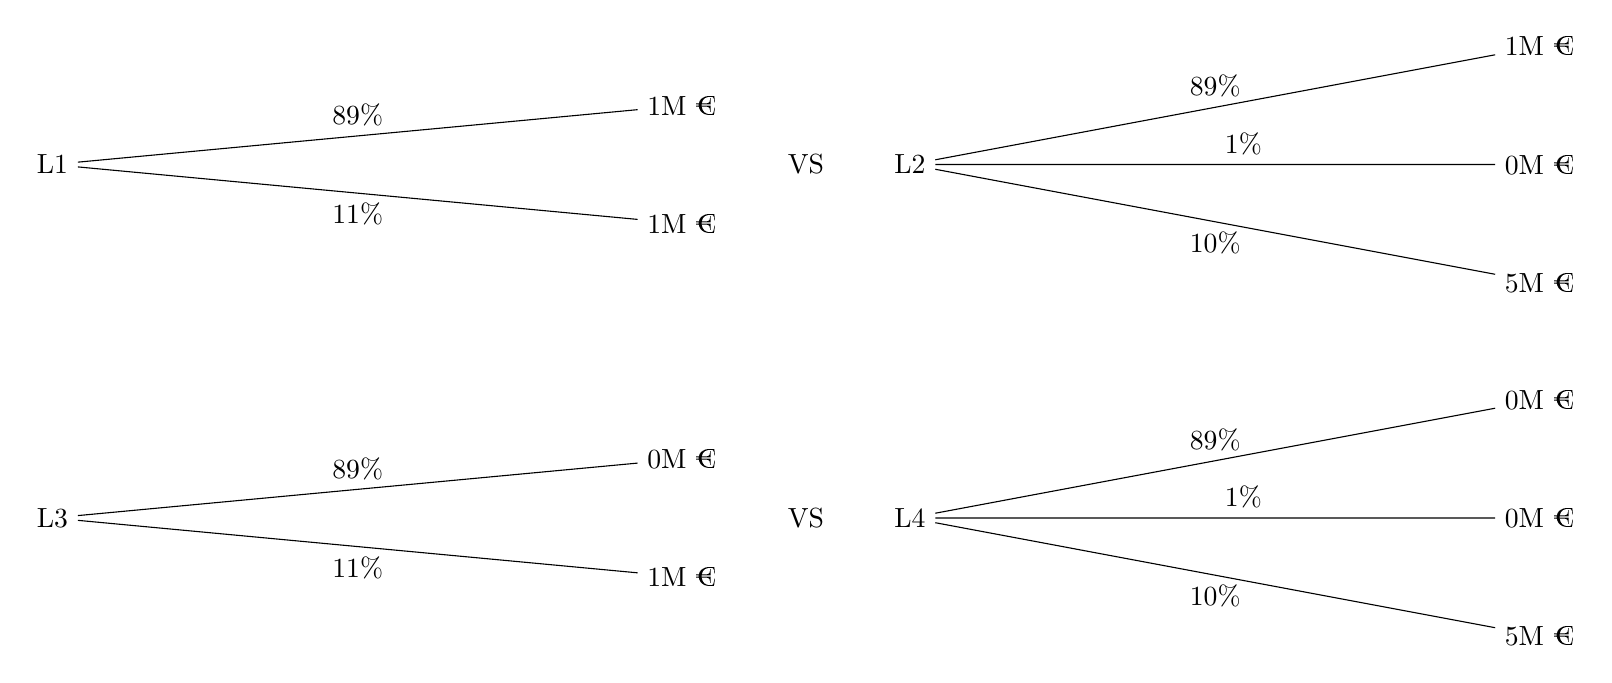
\begin{tikzpicture}[grow'=right, sibling distance=1.5cm, level distance=8cm]
			\path node (l1) {L1} child {
				node {1M €} edge from parent node[above] {89\%}
			} child {
				node {1M €} edge from parent node[below] {11\%}
			};
			\path (l1 -| l1-1.east) ++ (\seplott, 0) node (ql12) {VS};
			\path (ql12) ++ (\seplott, 0) node[anchor=west] (l2) {L2} child {
				node {1M €} edge from parent node[above] {89\%}
			} child {
				node {0M €} edge from parent node[above right] {1\%}
			} child {
				node {5M €} edge from parent node[below] {10\%}
			};
			\path (l1.south) ++(0, -4cm) node[anchor=north] (l3) {L3} child {
				node {0M €} edge from parent node[above] {89\%}
			} child {
				node {1M €} edge from parent node[below] {11\%}
			};
			\path (l3 -| l3-1.east) ++ (\seplott, 0) node (ql34) {VS};
			\path (ql34) ++ (\seplott, 0) node[anchor=west] (l4) {L4} child {
				node {0M €} edge from parent node[above] {89\%}
			} child {
				node {0M €} edge from parent node[above right] {1\%}
			} child {
				node {5M €} edge from parent node[below] {10\%}
			};
		\end{tikzpicture}
	\end{minipage}
}

\block{Study deliberated judgement}{
	The proposed research program aims at the following.
	\begin{itemize}
		\item Define \ac{DJ} formally
		\begin{itemize}
			\item Given a set of arguments
			\item Of an individual $i$
			\item[⇒] The position that is stable facing counter-arguments
		\end{itemize}
		\item Define the concept of a model of someone’s \ac{DJ}
		\begin{itemize}
			\item[⇒] A model phrases a claim about $i$’s \ac{DJ} and argues for its claim
		\end{itemize}
		\item Define validity of a model
		\begin{itemize}
			\item[⇒] Correct capture of $i$’s \ac{DJ}
		\end{itemize}
		\item Study conditions for falsifying models using observable data only
		\begin{itemize}
			\item[⇒] Let models debate, use $i$ as a judge
		\end{itemize}
	\end{itemize}
}

\begin{columns}
	\column{0.5}
		\block{Application: test axioms of decision theory}{
			\begin{itemize}
				\item Axioms considered appropriate normatively?
				\begin{itemize}
					\item But some (Allais, Ellsberg) disagree
				\end{itemize}
				\item Proposal: build models resting on those axioms
				\item Test models: their convincing power will give us indications about the reasonableness of the axioms for “normal” people (meaning, not scientists studying decision theory)
			\end{itemize}
		}
	\column{0.5}
		\block{Application: test conceptions of justice}{
			\begin{itemize}
				\item Philosophers have proposed sophisticated conceptions of justice (Rawls, Nozick, …)
				\item Individual’s shallow intuitions about justice are observed and used to confront Rawls or others (Experimental Social Choice)
				\item Proposal: study reactions of individuals to arguments of philosophers rather than just shallow intuitions
				\item Move towards Reflective equilibrium (Goodman, Rawls)
			\end{itemize}
		}
\end{columns}
\end{document}

